\begin{figure*}[t]
\centering
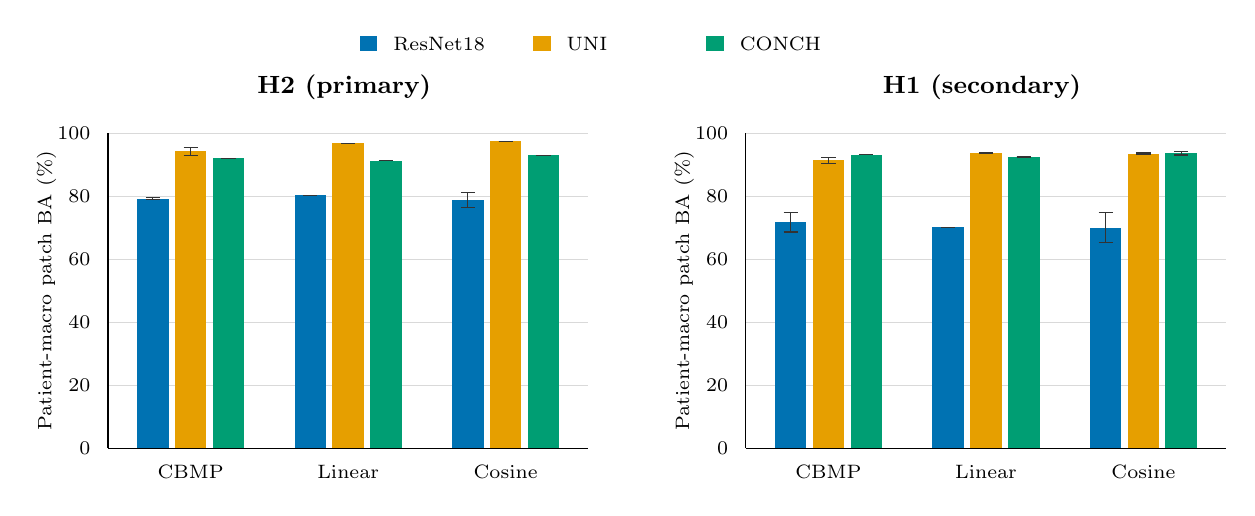
\begin{tikzpicture}[font=\scriptsize]
\definecolor{pathologyResnetBlue}{HTML}{0072B2}
\definecolor{pathologyUniOrange}{HTML}{E69F00}
\definecolor{pathologyConchGreen}{HTML}{009E73}
\fill[pathologyResnetBlue] (4.10,5.05) rectangle (4.32,5.23);
\node[anchor=west] at (4.40,5.14) {ResNet18};
\fill[pathologyUniOrange] (6.30,5.05) rectangle (6.52,5.23);
\node[anchor=west] at (6.60,5.14) {UNI};
\fill[pathologyConchGreen] (8.50,5.05) rectangle (8.72,5.23);
\node[anchor=west] at (8.80,5.14) {CONCH};
\begin{scope}[xshift=0.00cm]
\node[font=\small\bfseries] at (3.9,4.58) {H2 (primary)};
\draw[black!15] (.9,0.000) -- (7.0,0.000);
\node[anchor=east] at (.8,0.000) {0};
\draw[black!15] (.9,0.800) -- (7.0,0.800);
\node[anchor=east] at (.8,0.800) {20};
\draw[black!15] (.9,1.600) -- (7.0,1.600);
\node[anchor=east] at (.8,1.600) {40};
\draw[black!15] (.9,2.400) -- (7.0,2.400);
\node[anchor=east] at (.8,2.400) {60};
\draw[black!15] (.9,3.200) -- (7.0,3.200);
\node[anchor=east] at (.8,3.200) {80};
\draw[black!15] (.9,4.000) -- (7.0,4.000);
\node[anchor=east] at (.8,4.000) {100};
\node[rotate=90] at (.12,2) {Patient-macro patch BA (\%)};
\fill[pathologyResnetBlue] (1.270,0) rectangle (1.670,3.17150);
\draw[black!80] (1.470,3.15532) -- (1.470,3.18768);
\draw[black!80] (1.380,3.15532) -- (1.560,3.15532);
\draw[black!80] (1.380,3.18768) -- (1.560,3.18768);
\fill[pathologyUniOrange] (1.750,0) rectangle (2.150,3.76940);
\draw[black!80] (1.950,3.72146) -- (1.950,3.81734);
\draw[black!80] (1.860,3.72146) -- (2.040,3.72146);
\draw[black!80] (1.860,3.81734) -- (2.040,3.81734);
\fill[pathologyConchGreen] (2.230,0) rectangle (2.630,3.68443);
\draw[black!80] (2.430,3.68443) -- (2.430,3.68443);
\draw[black!80] (2.340,3.68443) -- (2.520,3.68443);
\draw[black!80] (2.340,3.68443) -- (2.520,3.68443);
\node at (1.950,-.30) {CBMP};
\fill[pathologyResnetBlue] (3.270,0) rectangle (3.670,3.21091);
\draw[black!80] (3.470,3.21091) -- (3.470,3.21091);
\draw[black!80] (3.380,3.21091) -- (3.560,3.21091);
\draw[black!80] (3.380,3.21091) -- (3.560,3.21091);
\fill[pathologyUniOrange] (3.750,0) rectangle (4.150,3.87129);
\draw[black!80] (3.950,3.87129) -- (3.950,3.87129);
\draw[black!80] (3.860,3.87129) -- (4.040,3.87129);
\draw[black!80] (3.860,3.87129) -- (4.040,3.87129);
\fill[pathologyConchGreen] (4.230,0) rectangle (4.630,3.65282);
\draw[black!80] (4.430,3.65282) -- (4.430,3.65282);
\draw[black!80] (4.340,3.65282) -- (4.520,3.65282);
\draw[black!80] (4.340,3.65282) -- (4.520,3.65282);
\node at (3.950,-.30) {Linear};
\fill[pathologyResnetBlue] (5.270,0) rectangle (5.670,3.15054);
\draw[black!80] (5.470,3.05401) -- (5.470,3.24707);
\draw[black!80] (5.380,3.05401) -- (5.560,3.05401);
\draw[black!80] (5.380,3.24707) -- (5.560,3.24707);
\fill[pathologyUniOrange] (5.750,0) rectangle (6.150,3.89578);
\draw[black!80] (5.950,3.89350) -- (5.950,3.89807);
\draw[black!80] (5.860,3.89350) -- (6.040,3.89350);
\draw[black!80] (5.860,3.89807) -- (6.040,3.89807);
\fill[pathologyConchGreen] (6.230,0) rectangle (6.630,3.71974);
\draw[black!80] (6.430,3.71747) -- (6.430,3.72201);
\draw[black!80] (6.340,3.71747) -- (6.520,3.71747);
\draw[black!80] (6.340,3.72201) -- (6.520,3.72201);
\node at (5.950,-.30) {Cosine};
\draw (.9,0) -- (7,0);
\draw (.9,0) -- (.9,4);
\end{scope}
\begin{scope}[xshift=8.10cm]
\node[font=\small\bfseries] at (3.9,4.58) {H1 (secondary)};
\draw[black!15] (.9,0.000) -- (7.0,0.000);
\node[anchor=east] at (.8,0.000) {0};
\draw[black!15] (.9,0.800) -- (7.0,0.800);
\node[anchor=east] at (.8,0.800) {20};
\draw[black!15] (.9,1.600) -- (7.0,1.600);
\node[anchor=east] at (.8,1.600) {40};
\draw[black!15] (.9,2.400) -- (7.0,2.400);
\node[anchor=east] at (.8,2.400) {60};
\draw[black!15] (.9,3.200) -- (7.0,3.200);
\node[anchor=east] at (.8,3.200) {80};
\draw[black!15] (.9,4.000) -- (7.0,4.000);
\node[anchor=east] at (.8,4.000) {100};
\node[rotate=90] at (.12,2) {Patient-macro patch BA (\%)};
\fill[pathologyResnetBlue] (1.270,0) rectangle (1.670,2.86932);
\draw[black!80] (1.470,2.74645) -- (1.470,2.99219);
\draw[black!80] (1.380,2.74645) -- (1.560,2.74645);
\draw[black!80] (1.380,2.99219) -- (1.560,2.99219);
\fill[pathologyUniOrange] (1.750,0) rectangle (2.150,3.65484);
\draw[black!80] (1.950,3.61478) -- (1.950,3.69490);
\draw[black!80] (1.860,3.61478) -- (2.040,3.61478);
\draw[black!80] (1.860,3.69490) -- (2.040,3.69490);
\fill[pathologyConchGreen] (2.230,0) rectangle (2.630,3.72858);
\draw[black!80] (2.430,3.72858) -- (2.430,3.72858);
\draw[black!80] (2.340,3.72858) -- (2.520,3.72858);
\draw[black!80] (2.340,3.72858) -- (2.520,3.72858);
\node at (1.950,-.30) {CBMP};
\fill[pathologyResnetBlue] (3.270,0) rectangle (3.670,2.80618);
\draw[black!80] (3.470,2.80618) -- (3.470,2.80618);
\draw[black!80] (3.380,2.80618) -- (3.560,2.80618);
\draw[black!80] (3.380,2.80618) -- (3.560,2.80618);
\fill[pathologyUniOrange] (3.750,0) rectangle (4.150,3.74981);
\draw[black!80] (3.950,3.74981) -- (3.950,3.74981);
\draw[black!80] (3.860,3.74981) -- (4.040,3.74981);
\draw[black!80] (3.860,3.74981) -- (4.040,3.74981);
\fill[pathologyConchGreen] (4.230,0) rectangle (4.630,3.69818);
\draw[black!80] (4.430,3.69818) -- (4.430,3.69818);
\draw[black!80] (4.340,3.69818) -- (4.520,3.69818);
\draw[black!80] (4.340,3.69818) -- (4.520,3.69818);
\node at (3.950,-.30) {Linear};
\fill[pathologyResnetBlue] (5.270,0) rectangle (5.670,2.80151);
\draw[black!80] (5.470,2.61208) -- (5.470,2.99094);
\draw[black!80] (5.380,2.61208) -- (5.560,2.61208);
\draw[black!80] (5.380,2.99094) -- (5.560,2.99094);
\fill[pathologyUniOrange] (5.750,0) rectangle (6.150,3.74166);
\draw[black!80] (5.950,3.73318) -- (5.950,3.75013);
\draw[black!80] (5.860,3.73318) -- (6.040,3.73318);
\draw[black!80] (5.860,3.75013) -- (6.040,3.75013);
\fill[pathologyConchGreen] (6.230,0) rectangle (6.630,3.74447);
\draw[black!80] (6.430,3.72349) -- (6.430,3.76546);
\draw[black!80] (6.340,3.72349) -- (6.520,3.72349);
\draw[black!80] (6.340,3.76546) -- (6.520,3.76546);
\node at (5.950,-.30) {Cosine};
\draw (.9,0) -- (7,0);
\draw (.9,0) -- (.9,4);
\end{scope}
\end{tikzpicture}
\caption{Equal-patient averages of patch balanced accuracy; these are not patient-diagnosis scores on the identical custom CAMELYON subset under four-candidate source-only selection. Bars show ten-seed means; whiskers show fitting-seed standard deviation, not patient- or hospital-population uncertainty. CBMP, linear logistic and trained cosine are prespecified views; all nine heads appear in the accompanying tables.}
\label{fig:pathology_encoders_patient_macro}
\end{figure*}
